
\chapter{Rys historyczny}
\label{sec:hisotryMap}

Pomimo że w obecnych czasach, mapy nie są niczym niezwykłym, i wydają się codziennością nie zawsze tak było. W histori człowieka można znaleść okresy czasu kiedy kartografia była nieznana, lub była bardzo niedokładna.

Pierwsze malowidła które można uznać za graficzną reprezentację otoczenia archeolodzy napotkali w okolicach Pavloc (Czechy), datowaną są one na 25 wiek przed naszą erą \cite{pre2} . Na 14 wiek p.n.e datowane są wykopaliska w Navarre(Hiszpania) obejmujące rysunki na piaskowcu \cite{pre1}.

Jeszcze w XIV kartografia była bardzo ograniczona, mapy którymi posługiwano się nie były zbyt dokłądne. 12 października 1410 gdy Krzysztof Kolumb dotarł do brzegów wyspy San Salvador uznaj ją za jedną z wysp japońskich \cite{columb}. Aby lepiej zrozumieć powód tej pomyłki wystarczy spojrzeć na mapę stworzoną w XV wieku przez kartografa Henricusa Martellusa \ref{fig:worldMap1}. Widzimy na niej że m.in. obie ameryki nie były znane uwczesnym ludzion.

\begin{figure}[H]
  \centering
    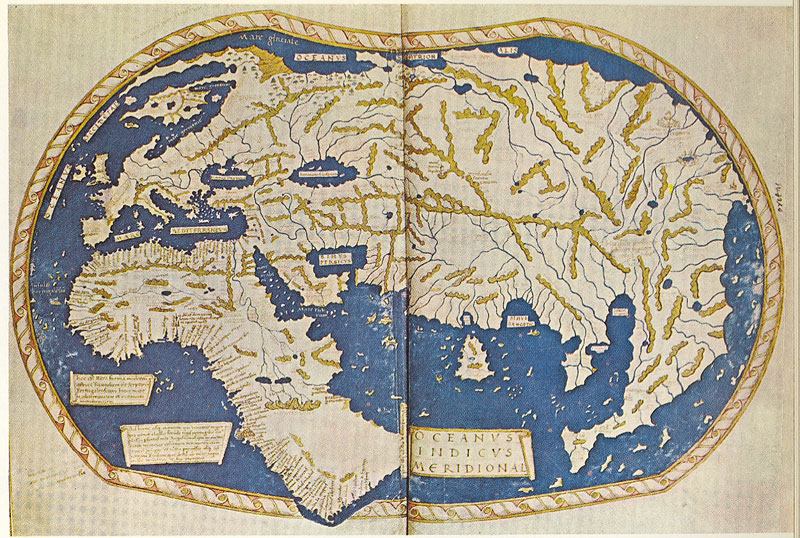
\includegraphics[width=100mm]{ge/worldMap1.jpg}
  \caption{Mapa świata z 1489 roku.}
  \label{fig:worldMap1}
\end{figure}

\chapter{Podstawy teoretyczne}
\label{cha:podstawyTeoretyczne}

\section{Rodzaje map}
\label{sec:Rodzaje map}

Tworząc aplikację która ma dostarczać informacji korzystających z map należy zapoznać się dostępnymi źródłami. Z powodu szrokiego wyboru poniżej omówione zostaną jedynie aplikacje które dostarczają informacji ogólnoświatowych. Na polskim rynku dostępnych jest kilka rozwiązań, ich główną wadą jest ograniczenie do terytorium Polski, dodatkowo często nie dostarczają one obrazów satelitarnych, są to m.in. \underline{\texttt{http://zumi.pl}}


\subsection{Google Maps}
\label{subsec:Google Maps}

Rysunek \ref{fig:googleMaps_1} przedstawia obraz otrzymany w aplikacji Google Maps. Dodatkowo włączona opcja prezentacji natężenia ruchu jedynie potwierdza duże możliwości i łatwość obsługi. Przyjazny interfejs sprawia że praca jest prosta i pozwala na osiągnięcie bardzo dobrych wyników.

\begin{figure}[H]
  \centering
    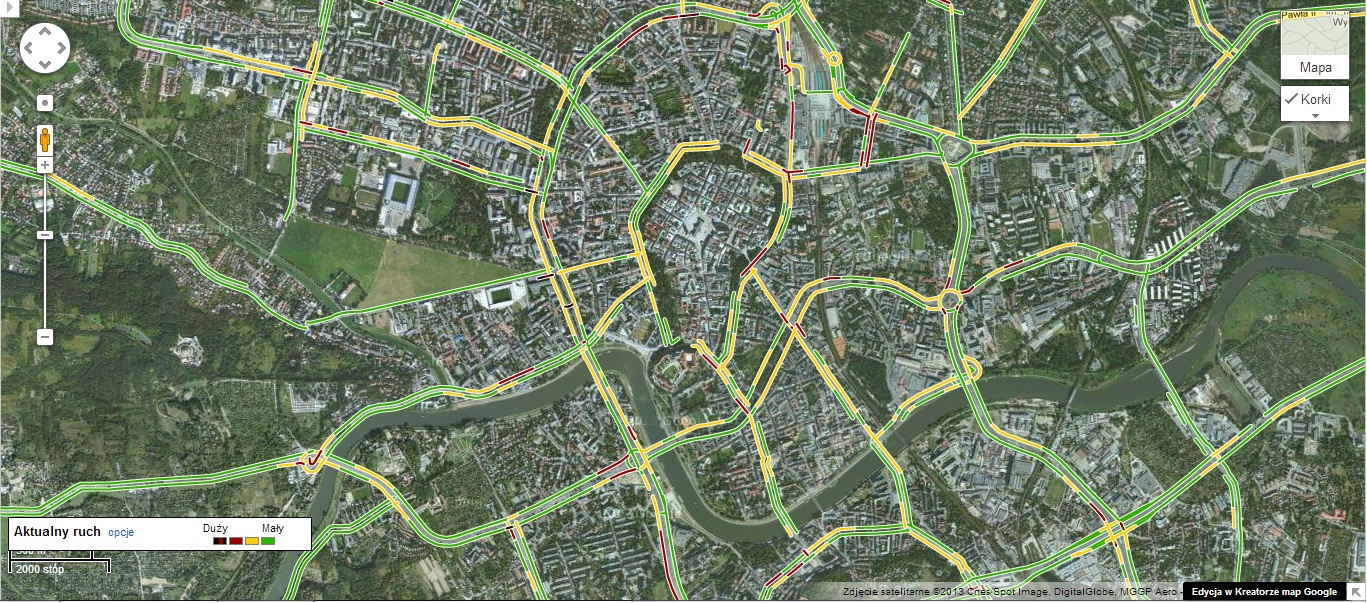
\includegraphics[width=100mm]{ge/gm_1.jpg}
  \caption{Google Maps.}
  \label{fig:googleMaps_1}
\end{figure}


\subsection{Windows Maps}
\label{subsec:Windows Maps}

Rysunek \ref{fig:bingMaps_1} przedstawia obraz otrzymany wykorzystując Bing Maps. W tym konkretnym przykładzie widzimy znaczną różnicę kolorów, obecność chmur pomniejsza wartość tych zdjęć. Należy wspomnieć o znacznie uboższym interfejsie dostarczanym użytkownikowi, interakcja jest w znacznym stopniu uboższa.

\begin{figure}[H]
  \centering
    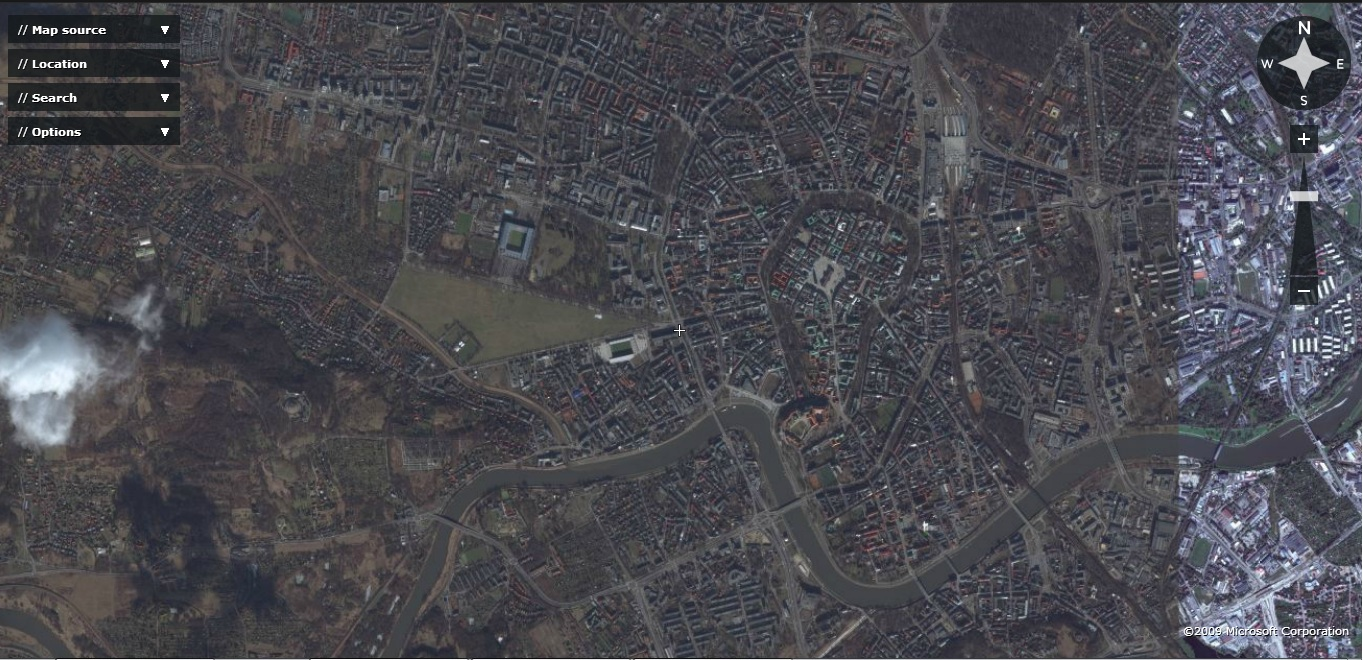
\includegraphics[width=100mm]{ge/bing_1.jpg}
  \caption{Bing Maps.}
  \label{fig:bingMaps_1}
\end{figure}

\subsection{Yahoo Maps}
\label{subsec:Yahoo Maps}

Kolejnym dostarczycielem danych kartograficznym jest Yahoo, przykład znajduje się na rysunku \ref{fig:yahooMaps_1}. Interfejs jest zbliżony do Bing Maps, jednak obszar na którym możemy przedlądać zdjęcia jest mniejszy, obszary oddalone od większych miast nie są w pełni uwzglęnione.

tylko granice krakowa

\begin{figure}[H]
  \centering
    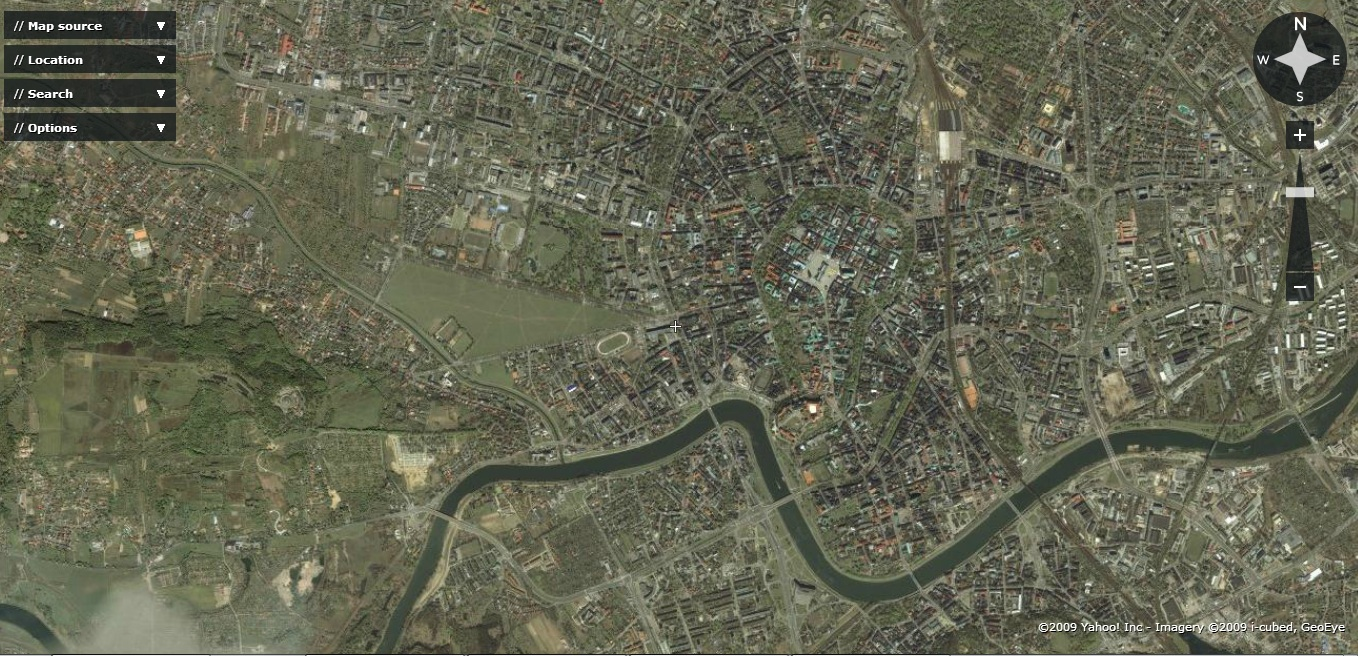
\includegraphics[width=100mm]{ge/yahoo_1.jpg}
  \caption{Yahoo Maps.}
  \label{fig:yahooMaps_1}
\end{figure}

\subsection{Apple Maps}
\label{subsec:Apple Maps}

Kolejną dużą marką która dostarcza informację jest Apple. Niestety nie ma wersji która pozwalałaby na dostęp do tej usługi z powszechnie używanych komputerów stacjonarnych.

\section{Google Earth}
\label{sec:Google Earth}

Ciekawe wykorzystanie obrazów satelitarnych i wskaźnika czasu zostało zaprezentowane w programie Google Earth. W aplikacji tej możemy zobaczyć nie tylko najbardziej aktualne zdjęcia, ale jesteśmy w stanie cofnąć się w czasie i zobaczyć jak wyglądał obszar na który patrzymy w przeszłości.

Przykład takiej sytuacji został przedstawiony na rysunku \ref{fig:lasVegas1}, obraz terenu na którym powstanie miasto Las Vegas w roku 1950. Jak teren ten wyglądał w roku 1977 widzimy na rysunku \ref{fig:lasVegas2}, pomimo widocznych zmian teren ten nadal w dużym stopniu jest pustynny,dopiero na rysunku \ref{fig:lasVegas3} widzimy aktualny stan miasta.

Dzięki funkcji zmiany punktu i kąta patrzenia, pokazywania ciekawych miejsc czy chociażby włączania trybu w którym budynki nabierają formy przestrzennej, 3D, możemy poprzez zabawę i wirtualne wycieczki poszeżać naszą wiedzę o otaczającym nas świecie.

\begin{figure}[H]
  \centering
    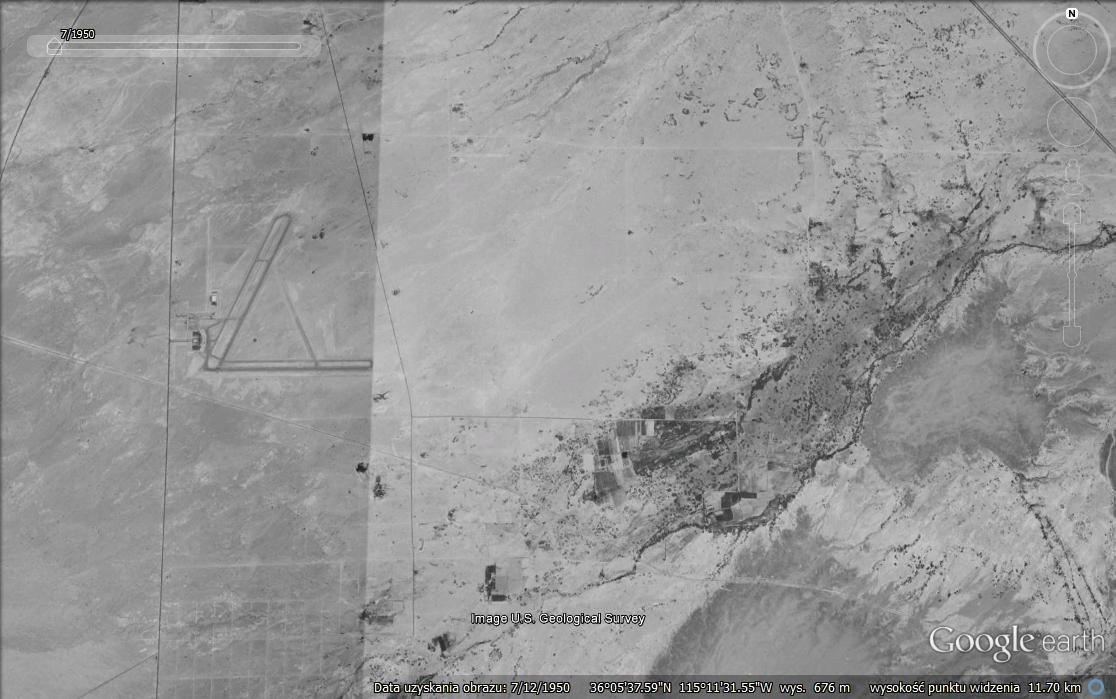
\includegraphics[width=100mm]{ge/01_1950.jpg}
  \caption{Las Vegas w 1950 roku.}
  \label{fig:lasVegas1}
\end{figure}

\begin{figure}[H]
  \centering
    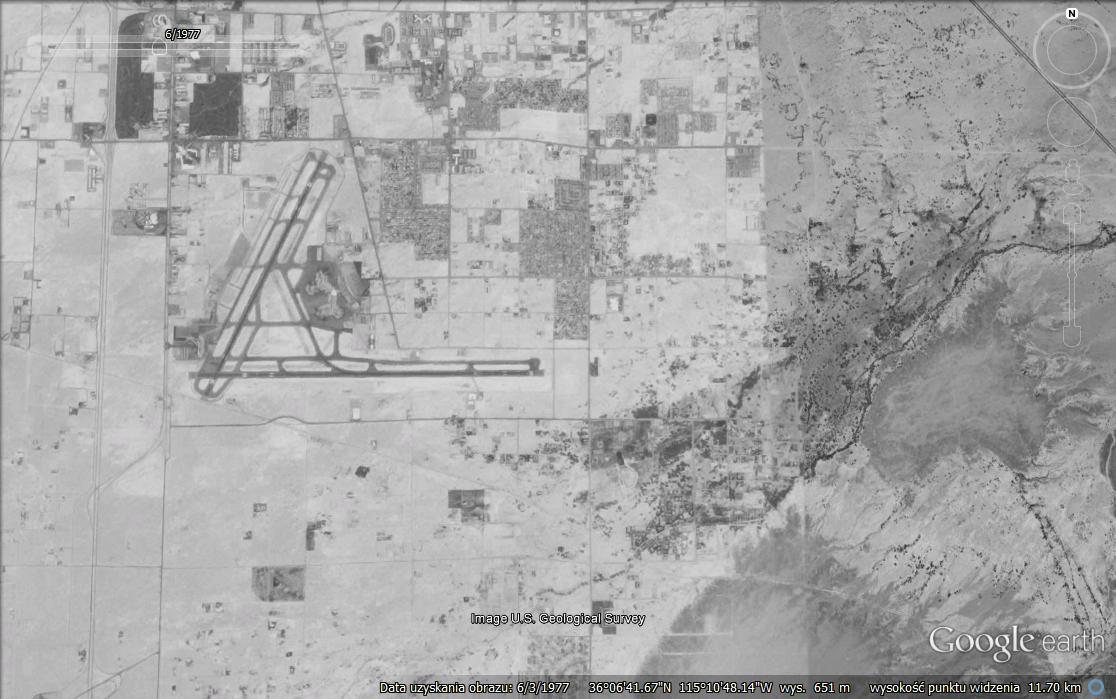
\includegraphics[width=100mm]{ge/02_1977.jpg}
  \caption{Las Vegas w 1950 roku.}
  \label{fig:lasVegas2}
\end{figure}

\begin{figure}[H]
  \centering
    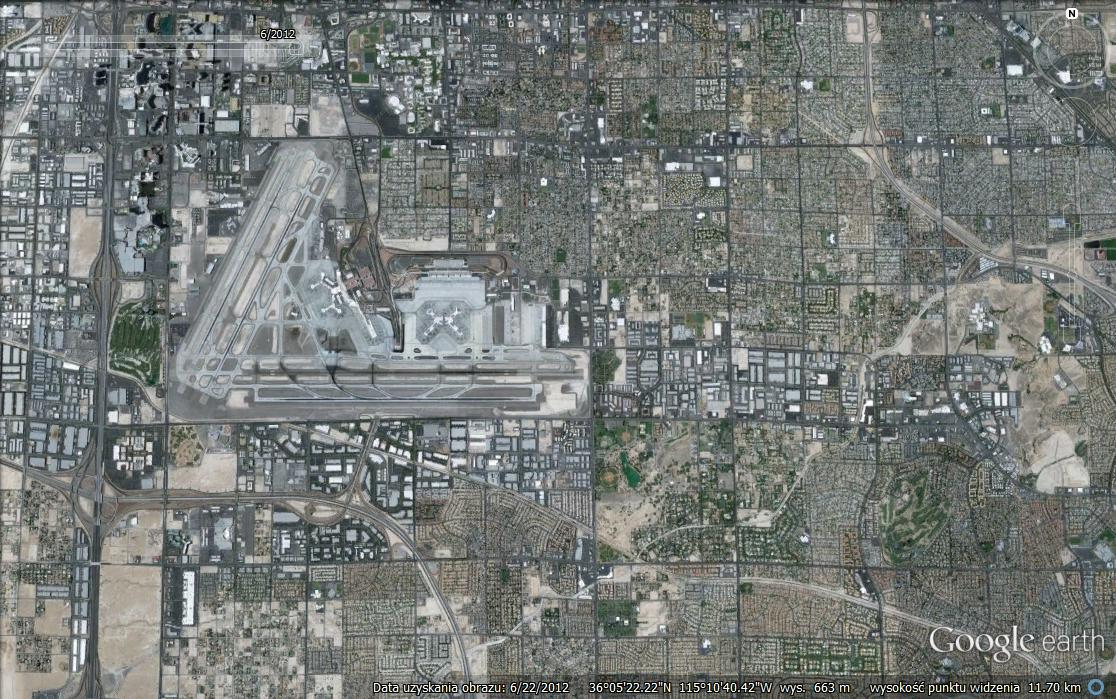
\includegraphics[width=100mm]{ge/03_2012.jpg}
  \caption{Las Vegas w 1950 roku.}
  \label{fig:lasVegas3}
\end{figure}

\section{Oś czasu}
\label{sec:osCzasu}

Jedną z większych uniedogonień podczas korzystania z map jest ich statyczność. Tradycyjne mapy pozwalają poznać jedynie jedną konkretną sytuację któa panowała na danym obszarze, nawet jeśli nałożymy kilka informacji z różnych okresów na jeden obraz, wynik może przestać być czytely. Korzystając w map dostępnych w internecie zazwyczaj istnieje opcja zmiany widoku. W jednej chwili możemy być na wysokości kilkuset kilometrów nad poziomem morza, aby w kolejnej znaleść się kilkaset metrów nad ziemią.

Ciekawą opcją jest dostarczana przez Google Earth możliwość zmiany czasu wykonania zdjęć. Niestety jest ona nieprzydatna jeśli chcemy przezentować własne dane.




